\setlength{\parskip}{\baselineskip} 
\section{Child IQ}

\begin{frame}
 \frametitle{Table of Contents}
 \vspace{-2em}
\textbf{
\begin{itemize}
 {\color{gray}
     \item {Background}}
     {\color{gray}
         \item PCP}
         \begin{itemize}
         {\color{gray}
             \item Method
             \item Simulations
             \item Application}
         \end{itemize}
          {\color{gray}
         \item \bnmf}
         \begin{itemize}
         {\color{gray}
             \item Method
             \item Simulations
             \item Application}
         \end{itemize}
    {\color{matbluedark}
     \item \bnmf \& Child IQ}
    {\color{gray}
     \item Conclusion
     }
 \end{itemize}}
\end{frame}

\frame{
\frametitle{Mixture exposure \textit{in utero}}
\begin{columns}
\column{.5\textwidth}
\begin{itemize}
    \item Exposure in humans unique to each individual
    \item Pregnant women especially vulnerable
    \item Gestation a critical period of brain development
    \item Prenatal exposures \aritem \  cognitive deficits in children
\end{itemize}
\column{.5\textwidth}
\vspace{-2em}
{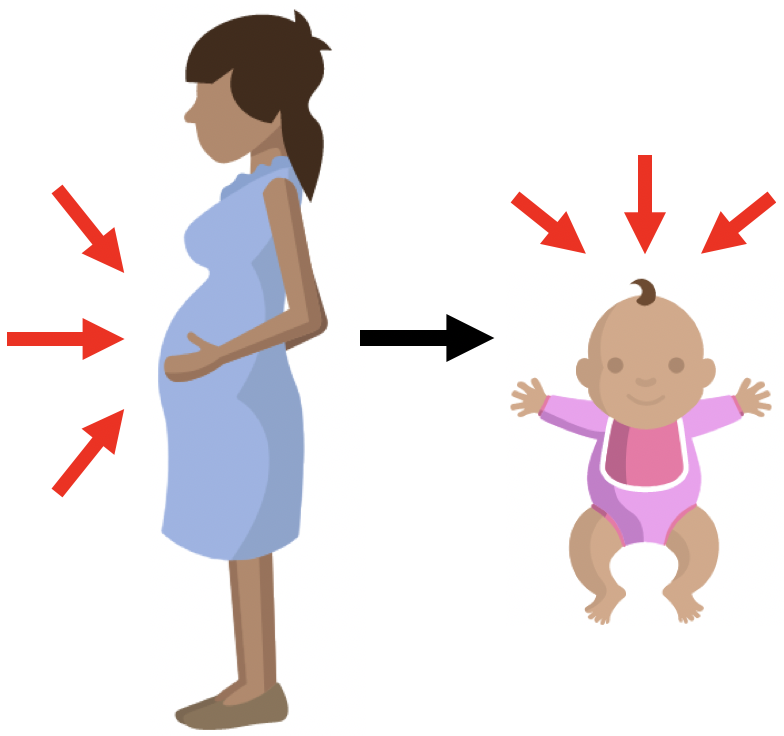
\includegraphics[scale = 0.35]{figures/bn2mf/baby.png}}
\end{columns}
}

\frame{
\frametitle{Mixture population-level effect}
%\vspace{-0.5em}
\begin{center}
{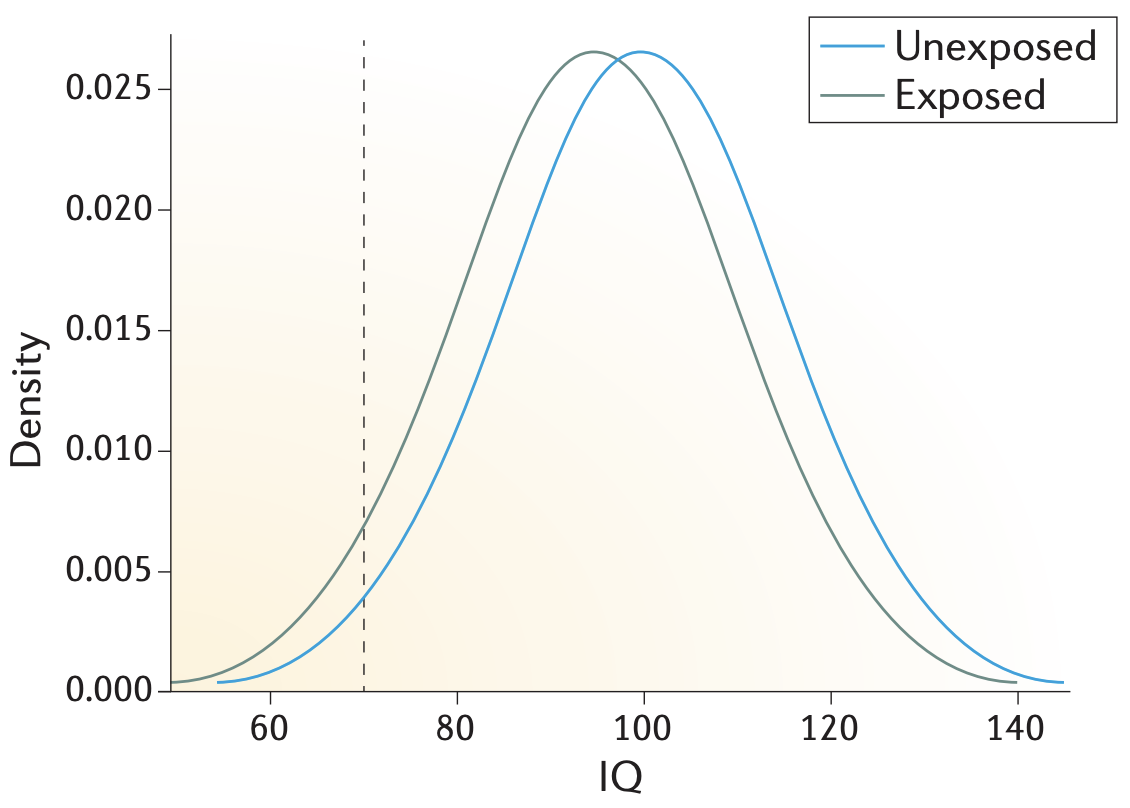
\includegraphics[scale = 0.39]{figures/bn2mf/braun.png}}
\end{center}
\vspace{-3.5em}
\begin{flushright}
\tiny{\color{hgray}{Braun et al., 2017}}\phantom{xxxxxxxxxxxxxxxxxx}
\end{flushright}
\vspace{-1.5em}
\hspace{1em}
\centering{\normalsize\textbf{\emph{Small downward shift has substantial population impact}}}
}

\frame{
\frametitle{Two-stage health model specifications}
\begin{itemize}
    \item {\color{matbluedark}\textbf{Outcome of interest:}} WISC-IV Full Scale Child IQ at age 7
    \item {\color{matbluedark}\textbf{Exposure of interest:}} \bnmfc-identified EDC patterns
    \item {\color{matbluedark}\textbf{Covariates:}} {\small Maternal age, IQ, education, prenatal alcohol consumption, marital status, HOME score, \& material hardship}
    \item {\color{matbluedark}\textbf{Sex-specific analysis}}
    \end{itemize}
}

\frame{
\frametitle{Two-stage health model specifications}
\centering\begin{tcolorbox}[colframe=matbluedark, colback=white,halign=center,width=9cm, height=1.25cm]
\only<1>{\vspace{-1.25em}$$Y_i = \beta_0 + \beta_Z Z_i + \beta_{S} S_i + \beta_{Z \cdot S} \left(Z_i S_i\right) + \mathbf{X}_{i}^T\boldsymbol{\beta}_\mathbf{X} + \varepsilon_i$$}
%%
\only<2>{\vspace{-1.25em}$$\mathcolorbox{yellow}{Y_i} = \beta_0 + \beta_Z Z_i + \beta_{S} S_i + \beta_{Z \cdot S} \left(Z_i S_i\right) + \mathbf{X}_{i}^T\boldsymbol{\beta}_\mathbf{X} + \varepsilon_i$$}
%%
\only<3>{\vspace{-1.25em}$$Y_i = \beta_0 + \mathcolorbox{yellow}{\beta_Z Z_i} + \beta_{S} S_i + \beta_{Z \cdot S} \left(Z_i S_i\right) + \mathbf{X}_{i}^T\boldsymbol{\beta}_\mathbf{X} + \varepsilon_i$$}
%%
\only<4>{\vspace{-1.25em}$$Y_i = \beta_0 + \beta_Z Z_i + \mathcolorbox{yellow}{\beta_{S} S_i} + \beta_{Z \cdot S} \left(Z_i S_i\right) + \mathbf{X}_{i}^T\boldsymbol{\beta}_\mathbf{X} + \varepsilon_i$$}
%%
\only<5>{\vspace{-1.25em}$$Y_i = \beta_0 + \beta_Z Z_i + \beta_{S} S_i + \mathcolorbox{yellow}{\beta_{Z \cdot S} \left(Z_i S_i\right)} + \mathbf{X}_{i}^T\boldsymbol{\beta}_\mathbf{X} + \varepsilon_i$$}
%%
\only<6>{\vspace{-1.25em}$$Y_i = \beta_0 + \beta_Z Z_i + \beta_{S} S_i + \beta_{Z \cdot S} \left(Z_i S_i\right) + \mathcolorbox{yellow}{\mathbf{X}_{i}^T\boldsymbol{\beta}_\mathbf{X}} + \varepsilon_i$$}
%%
\only<7>{\vspace{-1.25em}$$Y_i = \beta_0 + \beta_Z Z_i + \beta_{S} S_i + \beta_{Z \cdot S} \left(Z_i S_i\right) + \mathbf{X}_{i}^T\boldsymbol{\beta}_\mathbf{X} + \varepsilon_i$$}
\end{tcolorbox}
\vspace{-1ex}
\begin{itemize}
    \item {\color{matbluedark}\textbf{Traditional multivariable regression model}}
%\vspace{-1ex}
\begin{equation*}
\hspace{-6cm} Z_i = \mathbb{E}\left[\widehat{W}_i\times \widehat{\mathbf{a}}_i\right]
\end{equation*}
%\vspace{-1.5em}   
\item {\color{matbluedark}\textbf{Bayesian hierarchical model}}
\end{itemize}
\vspace{-0.8ex}
\begin{equation*}
\hspace{-1cm} Z_i \sim \operatorname{Gamma}(\widehat{\alpha}_{W i}, \widehat{\beta}_{W i}) \times \operatorname{Gamma}(\widehat{\alpha}_{\mathbf{a} i},\widehat{\beta}_{\mathbf{a} i})
\end{equation*}
}

\frame{
\frametitle{Are \bnmfc-identified patterns associated with child IQ?}
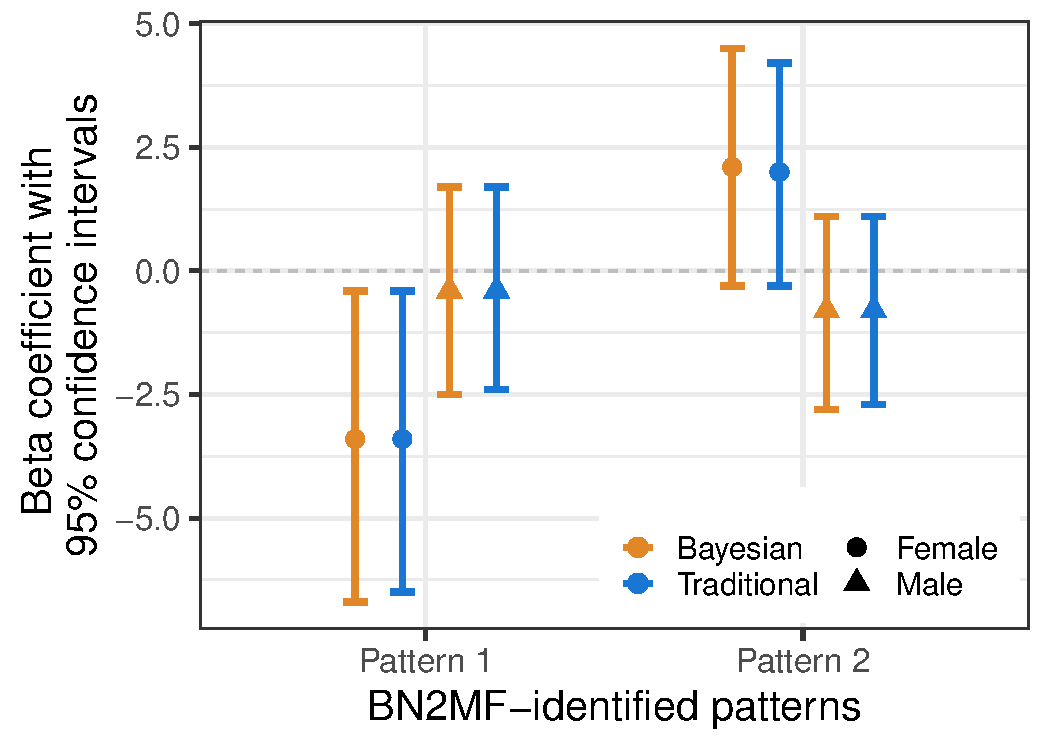
\includegraphics[scale=.57]{figures/bn2mf/modelplot.pdf}
}

\frame{
\frametitle{Are \bnmfc-identified patterns associated with child IQ?}
\begin{columns}
\column{.45\textwidth}

\includegraphics[scale=.2]{figures/yes-1.jpg}
\column{.55\textwidth}
\vspace{1em}
\begin{changemargin}{-1em}{0em}
\begin{itemize}
    \item Phthalate + BPA pattern associated with lower female IQ
    \begin{itemize}
        \item[\aritem] Joins large body of research
        \item[\aritem] EDC sex-specific effects on neurodevelopment
    \end{itemize}
    \item EDC exposure is \textit{modifiable}
    \begin{itemize}
        \item[\aritem] Easier to act on pattern than individual EDC
        \item[\aritem] Targeted public health and regulatory action
        \item[\aritem] Comprehensive regulation of chemicals that co-occur
    \end{itemize}
\end{itemize}
\end{changemargin}
\end{columns}
}

